% based on the CVPR template provided by Ming-Ming Cheng (https://github.com/MCG-NKU/CVPR_Template)
% modified and extended by Stefan Roth (stefan.roth@NOSPAMtu-darmstadt.de)

\documentclass[10pt,twocolumn,letterpaper]{article}

%%%%%%%%% PAPER TYPE
\usepackage[pagenumbers]{cvpr}

% Include other packages here, before hyperref.
\usepackage{graphicx}
\usepackage{amsmath}
\usepackage{amssymb}
\usepackage{booktabs}

% If you comment hyperref and then uncomment it, you should delete
% Hadley_Proposal.aux before re-running LaTeX.
% (Or just hit 'q' on the first LaTeX run, let it finish, and you
%  should be clear).
\usepackage[pagebackref,breaklinks,colorlinks]{hyperref}

% Support for easy cross-referencing
\usepackage[capitalize]{cleveref}
\crefname{section}{Sec.}{Secs.}
\Crefname{section}{Section}{Sections}
\Crefname{table}{Table}{Tables}
\crefname{table}{Tab.}{Tabs.}

\begin{document}

%%%%%%%%% TITLE
\title{CS 153 Project Proposal\\
Mapping the density of flowers on California buckwheat plants
}

\author{Alex Hadley\\
Harvey Mudd College\\
Claremont, CA\\
{\tt\small ahadley@hmc.edu}
}
\maketitle

% %%%%%%%%% ABSTRACT
% \begin{abstract}
%    The ABSTRACT is to be in fully justified italicized text, at the top of the left-hand column, below the author and affiliation information.
%    Use the word ``Abstract'' as the title, in 12-point Times, boldface type, centered relative to the column, initially capitalized.
%    The abstract is to be in 10-point, single-spaced type.
%    Leave two blank lines after the Abstract, then begin the main text.
%    Look at previous CVPR abstracts to get a feel for style and length.
% \end{abstract}

%%%%%%%%% BODY TEXT
\section{Motivation}

The motivation for this project is\dots

Proposed by Professor Matina Donaldson-Matasci at Harvey Mudd College.

Citation example~\cite{Potts}.

Another citation~\cite{Donaldson}.

Third citation~\cite{Donkersley}.

Fourth citation~\cite{Rzanny}.

\section{Methods}

The provided files include JPEG images taken by a drone, and corresponding JSON files that include annotations for the plants in the image. Each annotation includes a class (``EFRA'' for \textit{Eriogonum fasciculatum}) and a polygon representing the boundary of the plant. For an example, see Figure~\ref{fig:annotation}.

I have already been able to visualize the annotations by adapting code written by Tom Fu, one of Prof. Donaldson's research students.\footnote{\url{https://github.com/tommyfuu/flower_map_new/blob/master/scripts/visualizePolygons.py}} The next step will be to convert the polygons into masks in order to isolate the portion of the image to analyze.

Given that the flowers 

\begin{figure}[t]
  \centering
   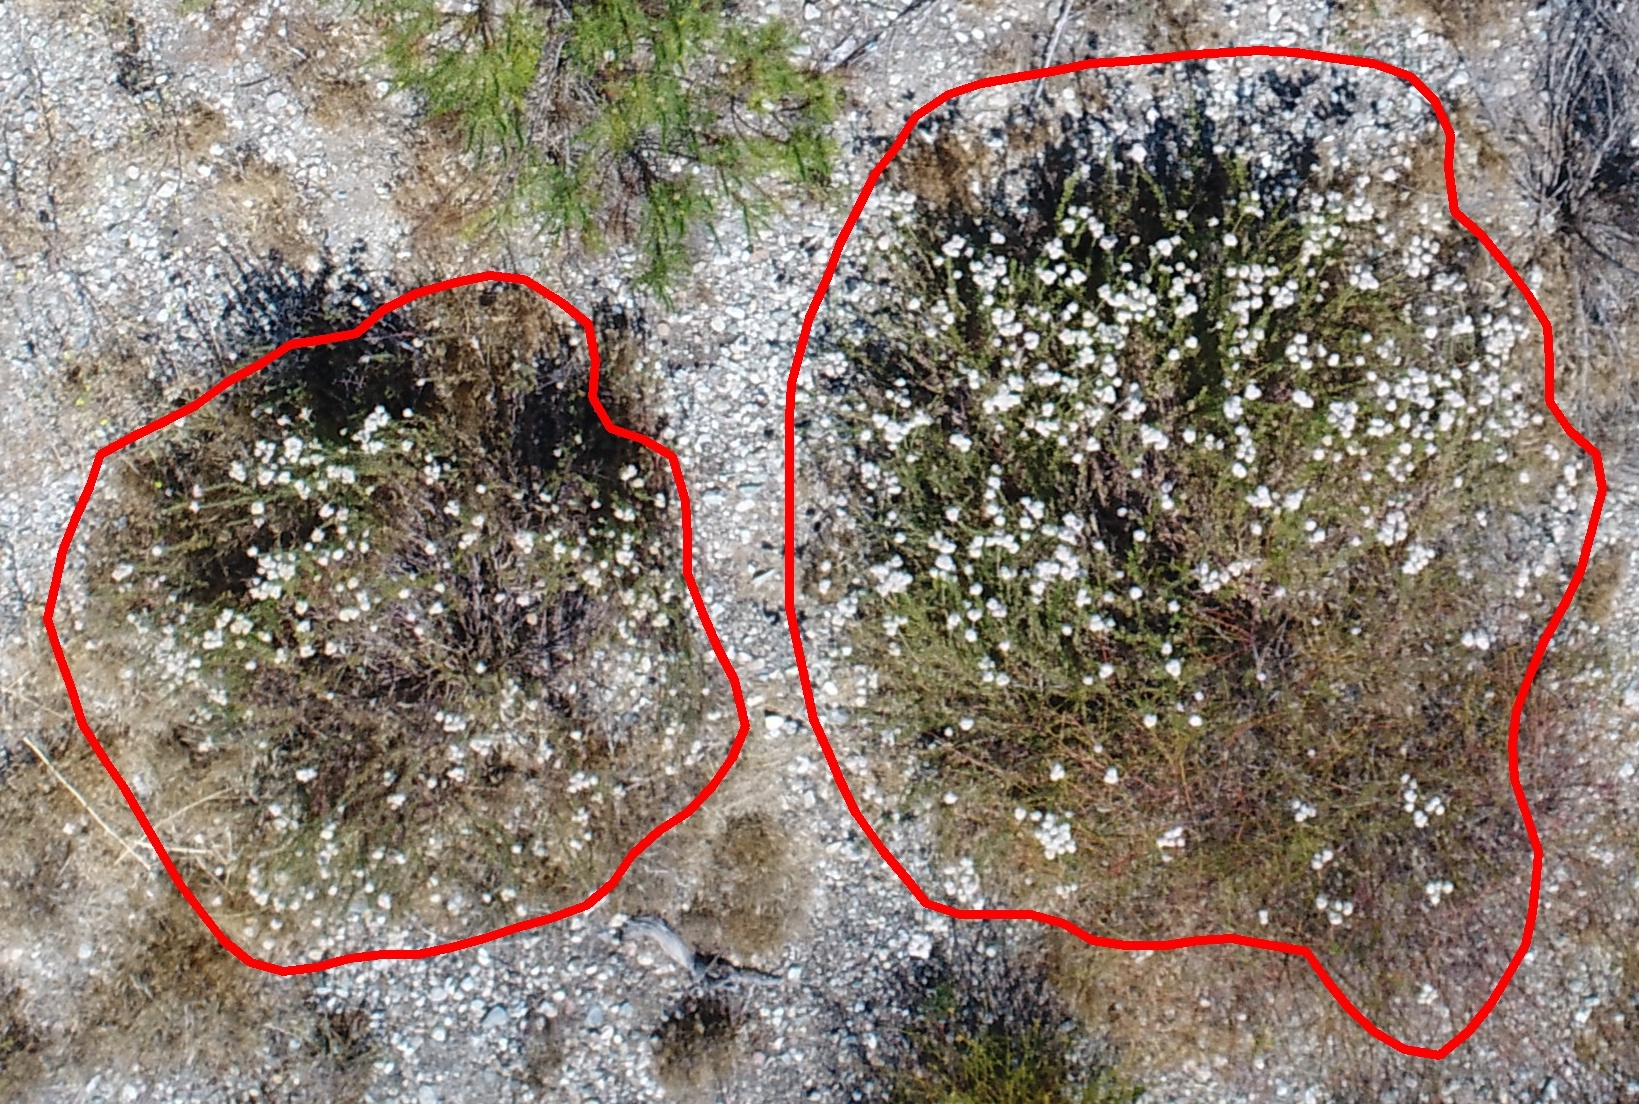
\includegraphics[width=0.9\linewidth]{annotation.jpg}
   \caption{An example of an included polygon annotation outlining a California buckwheat plant.}
   \label{fig:annotation}
\end{figure}

HSV thresholding, morphology, more ``classical'' approach

Mask R-CNN ??

Try thresholding as baseline, and Mask R-CNN, see if it can outperform thresholding.

\section{Measuring success}

Qualitative measure of the resulting masks
Precision, recall as compared to annotated data

\section{Challenges}

Annotating all of the data. Within the data provided, there are 888 images including California buckwheat plants, and across all images there are 11,981 individual plants. It will be a challenge to annotate the enough of these images to train and test a model well. There is no need to annotate all of the raw data, but it would be good to use some images from each batch.

The total size of the data is 9 GB, so it may be a challenge to store it all on Knuth or XSEDE. A caveat here is that for the purposes of training this model, we will only need to use the portions of the images within the annotation polygons.

%%%%%%%%% REFERENCES
{\small
\bibliographystyle{ieee_fullname}
\bibliography{egbib}
}

\end{document}
